\chapter{Generalised Linear Models}
\section{Examine distribution of G1, G2 and G3}
In this exercise we try to explain grades in mathematics of students by other predictive variables using linear models. First we have a look at the distribution of the dependent variables, here the first, second and third grade (G1, G2 and G3) during the year, to check whether a normal assumption is justified and we can use a standard linear model or whether we have to use a generalised linear model. Therefore we plot a histograms and QQ-Plots. Because the Poisson distribution seems suitable, too, for the data, we include a QQ-Plot for the normal distribution and the Poisson distribution (see Figure \ref{4gradedist}). 
\begin{figure}[ptb]
\centering
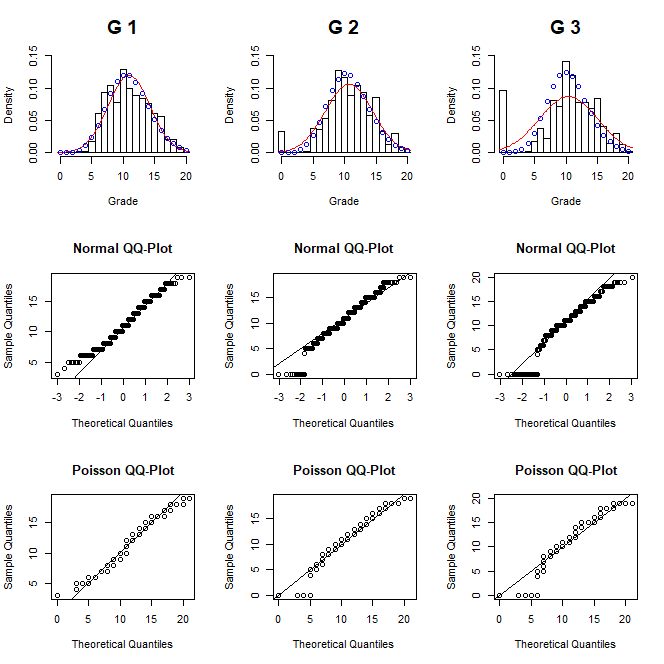
\includegraphics[width=\textwidth, keepaspectratio]{ex7/gradedist.png}
\caption{Histogram (first row) and QQ-Plots using Normal (second row) and Poisson (third row) distribution for theoretical quantiles for G1, G2 and G3. Red line represents the density of a fitted normal distribution and blue points a Poisson distribution, each with parameters estimated from the sample.}
\label{4gradedist}
\end{figure} 

Although the distributions look very similar, especially for G1 and G2, there are already some theoretical arguments that speak for the assumption of a Poisson distribution rather than a normal. First, the data is discrete, whereas the normal distribution has a density. Additionally the normal distribution allows negative numbers, too, whereas the Poisson distribution - although the values range trough $\mathbb{N}$ - only realises positive integer values. Still the data ranges only from 0 to 20, which is difficult to model reasonable with generalised linear models anyway. In the concrete data we see, that - especially for G3 - the Pisson distribution fits better to the data in the histogram. For G1 we see a rather good fit for both distributions. In the QQ-Plot we see that the sample distribution has shorter tails than the normal visible in the slightly S-curved shape of the plot, showing us that the sample quantiles at the border don't increase as fast as the theoretical at the right tail of the distribution an don't decrease that fast at the lower tail respectively. This pattern is less distinct for the Poisson distribution. Otherwise this would be a sign for underdispersion of the sample. The Fano factor $F$ is defined as the ratio of the variance over the mean of a distribution and equals 1 for a Poisson distribution. It is shown with other summary statistics in \ref{4tablegrades}. 
\begin{table}[ht]
\centering
\begin{tabular}{lrrrrrrrrr}
  \hline
 timepoint & min & q25 & med & M & q75 & max & IQR & SD & F \\ 
  \hline
   G1 &   3 &   8 &  11 & 10.91 &  13 &  19 &   5 & 3.32 & 1.01 \\ 
   G2 &   0 &   9 &  11 & 10.71 &  13 &  19 &   4 & 3.76 & 1.32 \\ 
   G3 &   0 &   8 &  11 & 10.42 &  14 &  20 &   6 & 4.58 & 2.02 \\ 
   \hline
\end{tabular}
\caption{Summary statistics for the grade (G1, G2, G3) in mathematics of the data set. Here $F$ is the Fano factor.}
\label{4tablegrades}
\end{table}

In the table we see that the Fano factor is near to one for G1 indicating that is there is no underdispersion. For G2 and G3 there is the problem of the high amount of 0 in the data, visible in the histogram and in the QQ-Plots as the first quantiles are all at 0. For G2 this is not that bad and the assumption of a Poisson distribution seems still justified because the rest of the data suits quite well. But also the normal distribution seems not far from the data. In the QQ-Plot we see that the points form a steeper curve compared to the reference line. This may be caused by the many zeros that don't suit to any of the both distributions. This is even more drastically for the third time point. Because the pattern is so much distorted, I decided to include the same plots for G3 where I dropped the zeros (see Figure \ref{4gradedist2}). There we see a much better in the histogram as well as in the QQ-Plots. Now a similar pattern as for G1 is visible. An underdispersion is also visible in the QQ-Plot for the Poisson distribution. The Fano factor for the reduced sample is now 0.90 indicating a slight underdispersion compared to a Poisson distribution, too. Without dropping zeros the Fano factor was 2.02 indicating a high overdispersion, which is quite obvious from the visualisations. Also for G2 the overdispersion was confirmed by a smaller Fano factor of 1.32, which is still greater than the optimum at 1. Summing up I would conclude that a Poisson distribution is theoretical more suitable and that the data follow its shape well enough to use generalised linear models.
\begin{figure}[thb]
\centering
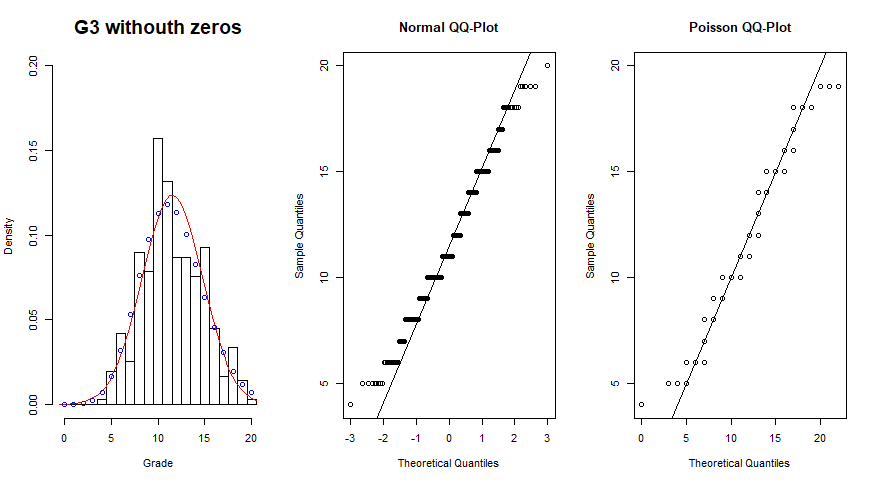
\includegraphics[width=\textwidth, keepaspectratio]{ex7/gradedist2.png}
\caption{Histogram and QQ-Plots for normal and Poisson distribution with sample parameters for G3 without zeros. The red line represents the fitted normal curve and blue points the Poisson distribution with sample mean.}
\label{4gradedist2}
\end{figure}	

\section{Model fit for G1}
Now we try to fit a suitable model to predict he first grade G1 from other variables. Those include for example sex, age and education and job of father and mother. With the function \texttt{glm} and the argument \texttt{family='poisson'} we fit a generalised linear model with a Poisson distributed response. The design matrix is built with all available independent variables. The reduced (I dropped some not significant variable in the list) output of the \texttt{summary} for the resulting \texttt{glm} object looks as follows:
% \newpage
\begin{small}\begin{verbatim} 
> summary(model1)

Call:
glm(formula = fmla, family = "poisson", data = dat)

Deviance Residuals: 
     Min        1Q    Median        3Q       Max  
-2.38057  -0.64611  -0.01502   0.50274   2.01602  

Coefficients:
                  Estimate Std. Error z value Pr(>|z|)    
(Intercept)       2.418107   0.331755   7.289 3.13e-13 ***
schoolMS          0.007157   0.058426   0.122  0.90250    
sexM              0.078237   0.036434   2.147  0.03176 *  
age              -0.006480   0.015983  -0.405  0.68515    
addressU          0.012823   0.043630   0.294  0.76882    
famsizeLE3        0.036639   0.035590   1.029  0.30325    
PstatusT          0.016047   0.053050   0.302  0.76227    
Medu              0.010664   0.023797   0.448  0.65405    
Fedu              0.014886   0.020349   0.732  0.46446    
Mjobhealth        0.078652   0.081444   0.966  0.33419    
[...]
traveltime       -0.003407   0.025788  -0.132  0.89488    
studytime         0.053887   0.020846   2.585  0.00974 ** 
failures         -0.147644   0.028151  -5.245 1.56e-07 ***
schoolsupyes     -0.211886   0.052610  -4.027 5.64e-05 ***
famsupyes        -0.093311   0.035213  -2.650  0.00805 ** 
paidyes          -0.008676   0.035007  -0.248  0.80426    
[...]
freetime          0.023120   0.017435   1.326  0.18482    
goout            -0.037487   0.016743  -2.239  0.02516 *  
Dalc             -0.002047   0.025074  -0.082  0.93494    
Walc             -0.004639   0.018663  -0.249  0.80371    
health           -0.015492   0.011868  -1.305  0.19178    
absences          0.001520   0.002185   0.696  0.48662    
---
Signif. codes:  0 `***` 0.001 `**` 0.01 `*` 0.05 `.` 0.1 ` ` 1

(Dispersion parameter for poisson family taken to be 1)

    Null deviance: 402.47  on 394  degrees of freedom
Residual deviance: 263.08  on 355  degrees of freedom
AIC: 2000.2

Number of Fisher Scoring iterations: 4
\end{verbatim}\end{small}  

There we see first some distributional measures for the deviance residuals. Let's have look at the coefficients. We see for each independent variable the estimate, standard error and z-value. In the last column there is the $p$ value. This indicated whether we consider the predictive value of a variable as significant or not. R indicates the usual threshold with the significance codes. Using this suggestion we see that most of the variables don't provide much predictive information about the grade. Just sex (\texttt{sexM}), weekly study time (\texttt{studytime}), number of past class failures (\texttt{failures}), extra educational support in school (\texttt{schoolsupyes}) and in the family (\texttt{famsupyes}) as well as the time a student goes out with friends (\texttt{goout}) are significant. Here a negative estimate indicates a negative influence for higher values or the level of the factor respectively. Male students (\texttt{sexM}) for example get higher grades (estimate 0.08) than female. Beneath the table for the coefficients we see the deviances. Testing the full model against the null model is quite needless here, since the full model will have a better fit to the data. Although we can check this very fast using the \texttt{anova} function in R after fitting the null model. The difference of deviances is 139.39 and thus significant ($p<.01$). A more interesting comparison to a nested model will be discussed in the next section. 

\begin{figure}[!h]
\centering
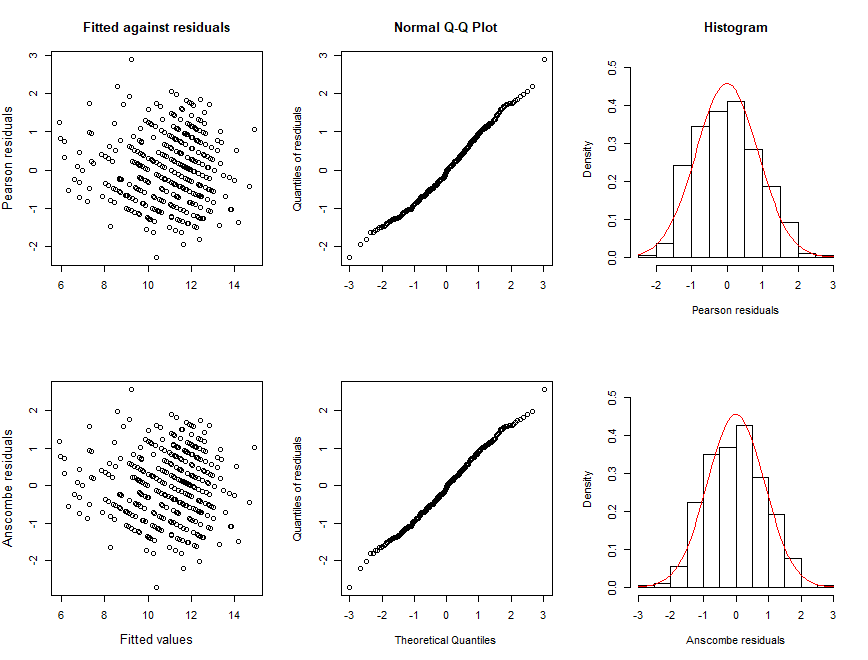
\includegraphics[width=\textwidth, keepaspectratio]{ex7/residuals.png}
\caption{Scatter plot for fitted values against residuals, QQ-Plot and histogram with fitted normal curve in red for Pearson residuals (first row) and Anscombe residuals (second row).}
\label{4resid}
\end{figure}

To examine the adequacy of the model we also have to look at the distribution of the residuals. There are many different approaches. The Pearson and Anscombe residuals are shown in Figure \ref{4resid}. An appropriate model will show normally distributed residuals. The Pearson residuals have to be taken with care, since for non-normal responses they are skewed. Therefore Anscombe resdiuals use a normalising transformation. Although both residual distribution look a little bit skewed in the histogram they show no obvious deviations in the QQ-Plot. The scatter plot on the left shows no systematic dependence from the height of the fitted values. All in all we may expect our model is a good choice for the data. 

\section{Reducing the model for G1}
We saw in the last section that most of our variables were not significant for the prediction in our full model. Therefore we fitted a reduced model containing the variables that were significant in the first model. Additionally we included the factor \texttt{Fedu} encoding the educational level of the father. The summary looks like follows:
\begin{small}\begin{verbatim} 
> summary(model2)

Call:
glm(formula = G1 ~ sex + Fedu + studytime + failures + schoolsup + 
    famsup + goout, family = "poisson", data = dat)

Deviance Residuals: 
     Min        1Q    Median        3Q       Max  
-2.70146  -0.70149  -0.02238   0.58681   2.55092  

Coefficients:
             Estimate Std. Error z value Pr(>|z|)    
(Intercept)   2.34585    0.07578  30.955  < 2e-16 ***
sexM          0.06585    0.03237   2.034  0.04193 *  
Fedu          0.04281    0.01482   2.888  0.00388 ** 
studytime     0.05828    0.01906   3.057  0.00223 ** 
failures     -0.13876    0.02495  -5.561 2.69e-08 ***
schoolsupyes -0.19834    0.04978  -3.984 6.78e-05 ***
famsupyes    -0.07330    0.03240  -2.263  0.02365 *  
goout        -0.03525    0.01406  -2.506  0.01220 *  
---
Signif. codes:  0 `***` 0.001 `**` 0.01 `*` 0.05 `.` 0.1 ` ` 1

(Dispersion parameter for poisson family taken to be 1)

    Null deviance: 402.47  on 394  degrees of freedom
Residual deviance: 302.02  on 387  degrees of freedom
AIC: 1975.1

Number of Fisher Scoring iterations: 4
\end{verbatim}\end{small}  

At first glance it may seem surprising that the variable \texttt{Fedu} is now significant. But since the whole model changes the estimates and standard errors for specific covariates change, too. Now we have a highly reduced model with only significant explaining variables. Compared to \texttt{model1} the residual deviance is of course higher. But the AIC, which is a criterion for the goodness-of-fit, which accounts for the size of the residuals as well as the number of coefficients to estimate in a model, decreased, indicating a better fit for \texttt{model2}. The residuals for \texttt{model2} follow a normal distribution, too. I omit the visualisation here since it is quite similar to the one in the last section, but it can be found in the supplementary code. Since the second model is nested in the full model we can compare them with an analysis of deviance. Like mentioned above this is easily done with the function \texttt{anova} and the argument \texttt{test='Chisq'}. With 32 degrees of freedom and a difference of 38.94 in the sum of residual deviances we get $p=.19$ indicating that the additional explaining value of the full model is not significant. Thus we can stick to the reduced model. 

A third model was fitted by dropping the variable \texttt{goout} and adding the variable \texttt{Walc} again: 
\begin{small}\begin{verbatim} 
> summary(model3)

Call:
glm(formula = G1 ~ sex + Fedu + studytime + failures + schoolsup + 
    famsup + Walc, family = "poisson", data = dat)

Deviance Residuals: 
     Min        1Q    Median        3Q       Max  
-2.64853  -0.69869  -0.02535   0.61090   2.51693  

Coefficients:
             Estimate Std. Error z value Pr(>|z|)    
(Intercept)   2.31120    0.07204  32.083  < 2e-16 ***
sexM          0.07558    0.03296   2.293  0.02183 *  
Fedu          0.04067    0.01477   2.753  0.00591 ** 
studytime     0.05231    0.01935   2.704  0.00685 ** 
failures     -0.14110    0.02488  -5.671 1.42e-08 ***
schoolsupyes -0.20115    0.04985  -4.035 5.46e-05 ***
famsupyes    -0.07447    0.03239  -2.299  0.02148 *  
Walc         -0.02614    0.01274  -2.052  0.04016 *  
---
Signif. codes:  0 `***` 0.001 `**` 0.01 `*` 0.05 `.` 0.1 ` ` 1

(Dispersion parameter for poisson family taken to be 1)

    Null deviance: 402.47  on 394  degrees of freedom
Residual deviance: 304.07  on 387  degrees of freedom
AIC: 1977.2

Number of Fisher Scoring iterations: 4
\end{verbatim}\end{small}  

There we see again that all covariates are significant and the residuals don't show serious deviations from the normal distribution (see code). Now, how can we tell, whether \texttt{model2} or \texttt{model3} is better? We can't use analysis of deviances here, since the two models are not nested. Therefore we have to keep at other measures, like penalised goodness-of-fit criteria (e.g. the AIC and BIC). Like mentioned above, a smaller AIC indicates a better fit. Since the two models estimated the same amount of coefficients, we don't need to use those but can directly look at the residual deviance or the likelihood. With a sum of 302.02 the second model is a bit better than the third one with 304.07. This is also visible in the difference of the log-likelihood. It is -979.57 for the second and -980.60 for the third model respectively. So \texttt{model2} has the higher likelihood and should hence be our choice. Still we have to keep in mind that this comparison is not inferential but descriptive. 